\documentclass{report}

\usepackage[english]{babel}

\usepackage[letterpaper,top=2cm,bottom=2cm,left=3cm,right=3cm,marginparwidth=1.75cm]{geometry}

\usepackage{amsmath}
\usepackage{graphicx}
\usepackage{tikz}
\usetikzlibrary{arrows}
\usetikzlibrary{arrows.meta,bending,chains}
\newcommand{\diff}{\mathop{}\!\mathrm{d}}
\usepackage[colorlinks=true, allcolors=blue]{hyperref}
\usepackage{imakeidx}
\usepackage{pgfplots}
\usepackage{hyperref}
\usepackage{bookmark}
\usepackage{booktabs}
\usepackage{pgfgantt}
\usepackage{multirow}
\usepackage{lscape}
\bookmarksetup{
  numbered,
  open
}
\pgfplotsset{width=10cm,compat=1.9}
\newcommand{\quantities}[1]{%
  \begin{tabular}{@{}c@{}}\strut#1\strut\end{tabular}%
}



\makeindex[columns=3, title=Alphabetical Index, intoc]

\title{Progetto e PMBOK}
\author{Lorenzo Sanseverino 5DSA}
\renewcommand*{\thesection}{\arabic{section}}


\begin{document}
\tableofcontents
\maketitle


\section{Definizione Di Progetto}

In ambito lavorativo ed aziendale un progetto è uno sforzo \textcolor{red}{temporaneo} intrapreso con lo scopo di crearea un \textcolor{red}{prodotto/servizio} unico e di qualità.
Ogni progetto intrapreso da una azienda \textbf{deve} ogni volta produrre sempre qualcosa di diverso. 

\subsection{Elemetti di un progetto e triangolo dal triplice vincolo}
In un progetto è solito trovare quattro elemetti in comune, su cui si baserà tutto lo sviluppo dello stesso, essi sono:

\begin{itemize}
\item Obiettivo
\item Scadenza
\item Unicità
\item Personale ed impiego delle risorse umane
\end{itemize}

In oltre, è solito fare riferimento al triangolo dal triplice vincolo.
\begin{figure}[h]
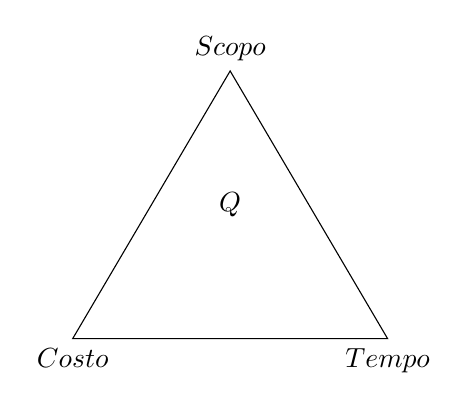
\begin{tikzpicture}
    \draw (0,0) node[anchor=north]{$Costo$}
        -- (4,0) node[anchor=north]{$Tempo$}
        -- (2,3.4) node[anchor=south]{$Scopo$}
        -- cycle    
        (2, 1.7) node[anchor=center]{$Q$};
\end{tikzpicture}
\caption{Triangolo dal triplice vincolo}
\label{t}
\end{figure}
Come è possibile visualizzare, nel caso in cui si dovesse dare più importanza ad uno di questi vincoli il triangolo non sarebbe più equilatero e bisognerebbe andare ad investire/magari perdere tempo per ri-aggiustarlo.
Molte volte è possibile trovare al centro una Q di Quality, questo fa riferimento ad una politica aziendale del cliente soddisfatto, \textit{\textcolor{red}{Total Quality Management}}, ossia si da la massima attenzione alla qualità del prodotto e ad offrire servizi ai clienti.

\section{Definizione di PMBOK e Project Management}
Il project Management esiste, se pur in forma primordiale, sin dai tempi degli antichi egizi e romani(le piramidi ed il Colosseo), le cui costruzione sarebbero state impossibile senza un profondo studio e organizzazione.
Nell'ultimo secolo il concetto di progetto si è diffuso sempre di più nelle varie aziende, e ciò ha portato alla necessità di metodologie per gestirlo, basti pensare a \textbf{Henry Gantt} nel '900 ed al suo diagramma a barre, che prende proprio il suo nome.
\begin{figure}[h]
\begin{ganttchart}{1}{12}
\gantttitle{2020}{12} \\
\gantttitlelist{1,...,12}{1} \\
\ganttgroup{Gruppo 1}{1}{7} \\
\ganttbar{Task 1}{1}{2} \\
\ganttlinkedbar{Task 2}{3}{7} \ganttnewline
\ganttmilestone{Milestone}{7} \ganttnewline
\ganttbar{Final Task}{8}{12}
\ganttlink{elem2}{elem3}
\ganttlink{elem3}{elem4}
\end{ganttchart}
\caption{Diagramma di Gantt}
\end{figure}

I motivi della sua diffusione sono tanti e ben distinti, ma possono essere riassunti in tre punti:
\begin{itemize}
    \item \textbf{Attività su commessa}
    \item \textbf{Problemi una tantum}
    \item \textbf{Strumento di innovazione}
\end{itemize}
La gestione del progetto attualemte è una vera e propria disciplina che prende il nome di \textbf{Project Management}.
Come concetti base della disciplina si può parlare di \textbf{CPM} (Critical Path Method, ossia di lavorare nella peggiore delle ipotesi per essere pronti ad ogni evenienza), il \textbf{PERT} (Program Evalutation and Review Tecnique, ossia valutare tempo e costo in rapporto ai rischi) ed il diagramma di \textbf{Gantt} (Utile per la gestione del tempo tramite piccole scadenze prefissate).
Tutto ciò viene descritto e ben spiegato nel \textbf{Project Management Body of Knowledge} che consiste in una vera e propria guida manageriale che ha lo scopo di definire linee guida per la gestione ed elaborazione di un progetto.

\subsection{Aree di Gestione}
Per descrivere le linee guida della gestione del progetto il PMBOK fa riferimento a 10 aree di gestione da membri diversi del gruppo.
\begin{enumerate}
    \item Gestione dell'ambito
    \item Gestione dei tempi
    \item Gestione dei costi
    \item Gestione della qualità
    \item Gestione delle risorse umane
    \item Gestione della comunicazione
    \item Gestione del rischio
    \item Gestione delle forniture
    \item Gestione delle integrazione dei processi
\end{enumerate}

\section{Figure del Project Management}

Le figure di un progetto e ciò che gli stessi devono fare/pensare può essere schematizzato con questo schema:

\begin{figure}[h!]
\begin{center}
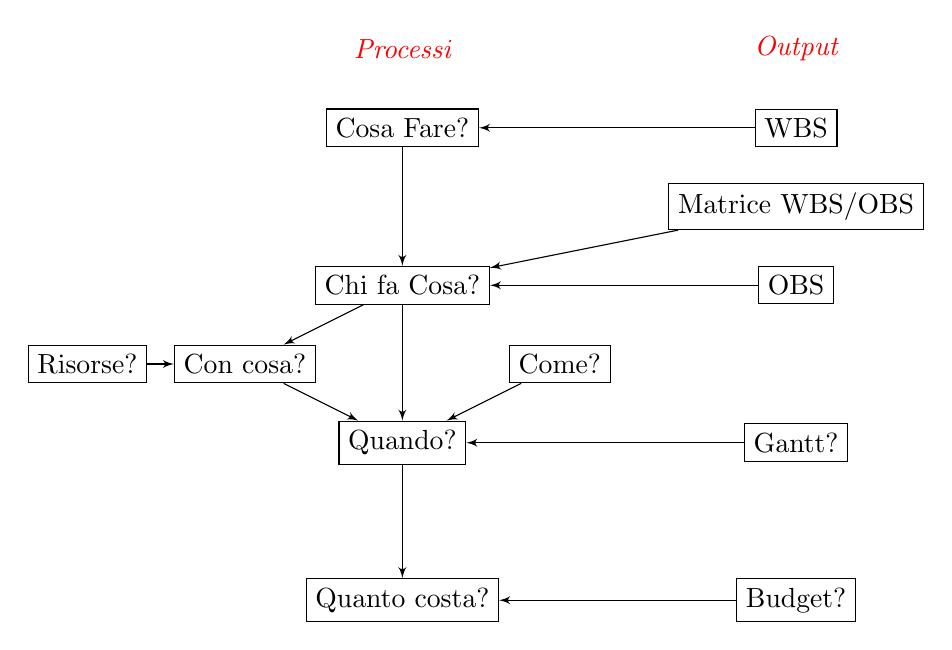
\begin{tikzpicture}
\node at (0, 1) {\textit{\textcolor{red}{Processi}}};
\node at (5, 1) {\textit{\textcolor{red}{Output}}};

\node[draw, rectangle] (s1) at (0,0) {Cosa Fare?};
\node[draw, rectangle] (t1) at (5,0) {WBS};

\node[draw,rectangle] (s2) at (0,-2) {Chi fa Cosa?};
\node[draw,rectangle] (t2) at (5,-2) {OBS};
\node[draw,rectangle] (t21) at (5,-1) {Matrice WBS/OBS};

\node[draw,rectangle] (s3) at (-2,-3) {Con cosa?};
\node[draw,rectangle] (t3) at (2,-3) {Come?};
\node[draw,rectangle] (t31) at (-4,-3) {Risorse?};


\node[draw,rectangle] (s4) at (0,-4) {Quando?};
\node[draw,rectangle] (t4) at (5,-4) {Gantt?};

\node[draw,rectangle] (s5) at (0,-6) {Quanto costa?};
\node[draw,rectangle] (t5) at (5,-6) {Budget?};
\path
    (t1) edge[->, >=latex', ] (s1)
    (s1) edge[->, >=latex', ] (s2)
    (t2) edge[->, >=latex', ] (s2)
    
    (s2) edge[->, >=latex', ] (s3)
    (s4) edge[->, >=latex']   (s5)
    (t31) edge[->, >=latex'] (s3)
    
    (t21) edge[->, >=latex',] (s2)
    (s3)  edge[->, >=latex'] (s4)
    (t3)  edge[->, >=latex'] (s4)
    (s2)  edge[->, >=latex'] (s4)
    (t4) edge[->, >=latex', ] (s4)
    (t5) edge[->, >=latex', ] (s5);
\end{tikzpicture}
\end{center}
\label{Schema}
\caption{Schema organizzativo}
\end{figure}
\textbf{WBS}: Work Breakdown Structure\\
\textbf{OBS}: Organizational Breakdown Structure\\
In una azienda, a gestire l'organizzazione e lo sviluppo di un progetto, è possibile trovare svariate figure che variano a seconda del tipo di azienda e progetto.
Una figura in comune per il Project Management è sicuramente quella del \textbf{Project Management}.
È la figura più importante, definito anche regista del progetto o, per citare Steve Jobs <<"I play the orchestra">>, il direttore dell'orchestra.
Lui non si preoccupa delle competenze tecniche ma di supervisione e coordinare tutti i membri del gruppo.
Si occupa di individuare la struttura di un progetto e di avviarla rispettando i vincoli (vedi Fig \ref{t}), deve organizzare un sistema di monitoraggio, una documentazione e cosa più importante prendere decisione sul \textbf{Make Or Buy}.

\section{Gestione del progetto in Ambito informatico}
\subsection{Definizione di Software}
La scrittura di un software non è una cosa così semplice come possa sembrare.
Dietro ogni software(per definizione "il linguaggio che sussurra all'hardware cosa fare) è presente uno sforzo quasi maggiore per la progettazione dello stesso che nella scrittura.
Il software si differenzia da un programma, in quando il software è progettato per essere duraturo nel tempo(ed aggiornato), ha una propria documentazione(es. Javadoc o i file ReadMe.md) è richiede uno sviluppo molto più costoso ed impegnativo. 
Questa materia, lo studio del software, prende proprio il nome di \textbf{Ingegneria del Software}.
\subsection{Software Engineering}
Come in ogni progetto, è presente il Project Manager che, in ambito informatico, prende proprio il nome di \textbf{Software Engineer} in quanto lui non si occupa di scrivere il codice ma di elaborare i vari modelli logici e concettuali, scegli  il linguaggio di programmazione, l'architettura della macchina ecc.
L'ingegneria del software, secondo la definizione di Dave Parnas, è "la costruzione di un software fatto di molte versione scritto da molte persone".
Si basa sul principio che lo sviluppo di un software è un'opera congiunta, ossia composta da molte persone che svolgono compiti diversi, e sul concetto di Evoluzione.
Un software per sua natura tende ad evolversi, o aggiornarsi, per riscontrarsi con le esigenze degli utenti.	
\subsection{Definizione di Ingegneria}
L'ingegneria si basa su tre aspetti fondamentali:
\begin{enumerate}
	\item Design: la ricerca di una soluzione dato un problema, sempre rispettando i vari vincoli.
	
	\item Costruzione: bisogna avere una idea precisa dei vari obiettivi che deve essere costruita in vari passaggi. Bisogna \textbf{monitorare}(verificare se tutto avviene secondo quanto stabilito) e \textbf{controllare}(intervenire in caso di errori).
	
	\item Operatività: una volta che i sistemi sono stati creati bisogna trovare delle soluzione economiche e fattibili.
	Per esempio, se si vende un software per la gestione di una libreria, tutti i vari database non possono essere salvati in una macchina in locale ma andrebbe usato un server esterno, in prevenzione di qualsiasi problema.
\end{enumerate}
\end{document}